%!TEX encoding = UTF-8 Unicode
% !TeX spellcheck = en_GB

%%%%%%%%%%%%%%%%%%%%%%%%%%%%%%%%%%%%%%
\chapter{ Optimised search for Higgs pair via Interpretable machine learning }\label{chap:overviewLightYuk}
%%%%%%%%%%%%%%%%%%%%%%%%%%%%%%%%%%%%%%
\section{Overview of Light Yukawa searches}
There are additional measurements of the light-quark Yukawa couplings that might become relevant at HL-LHC or FCC-hh, a careful study of which is beyond the scope of the current work. Yet we attempt to include a discussion here, so as to provide a comparison with our study and to put it into proper context, or to serve as proposal for further studies.

The channel $pp \to h +j $ has been suggested as a probe for charm Yukawa coupling~\cite{Brivio:2015fxa} with charm-tagged jet having a potential bound of $\kappa_c\sim 1$ for the HL-LHC, depending on the charm-tagging scheme. This process could be used for the first and second generations Yukawa couplings by looking at the shapes of kinematic distributions, the most important one being the $p_T$ distribution~\cite{Soreq:2016rae,Bishara:2016jga, Bonner:2016sdg}. The expected HL-LHC 95\% CL bounds are $\kappa_c \in [-0.6,3.0]$, $|\kappa_u |\lesssim 170 $ and $|\kappa_d| \lesssim 990$. The use of $h+j$ process along with other single Higgs processes have also been suggested as indirect probes for Higgs self coupling~\cite{McCullough:2013rea,Gorbahn:2016uoy,Bizon:2016wgr,Degrassi:2016wml,Maltoni:2017ims,Degrassi:2021uik}, due to the contribution of the trilinear coupling to NLO electroweak corrections to these processes. In addition, experimental fits have been carried out for the trilinear coupling from single Higgs observables~\cite{CMS:2018rig,ATLAS:2019pbo}. 

It seems that for the HL-LHC, an optimal bound for the trilinear coupling can be obtained by combing both the data from single-Higgs process as well as Higgs pair production~\cite{DiVita:2017eyz}, with 68\% CL bound on $\kappa_\lambda \in[0.1,2.3]$, compared to the expected bound of $\kappa_\lambda \in [0.0,2.5] \cup [4.9,7.4]$ coming from using di-Higgs measurements alone. Moreover, single Higgs processes, namely $Zh$ and $ W^\pm h$ production, could also be useful in probing charm-Yukawa coupling using a mixture of $b$- and $c$-tagging schemes leveraging the mistagging probability of $c$-jets as $b$-jets in $b$-tagging working points, and vice-versa, in order to break the degeneracy in the signal strength~\cite{Perez:2015lra}. The use of this technique could probe $\kappa_c \sim 1$ in the FCC-hh. Of course, for the charm-Yukawa coupling, the constraints are set to improve significantly, as there has been recent direct observation of $h\to c \bar c$~\cite{ATLAS-CONF-2021-021}. Therefore, from here on, we will mainly concentrate  on the process with more potential for constraining Yukawa couplings of the first generation quarks. 

Rare Higgs decays to mesons, $h \to M +V ,\, \, M = \Upsilon, J/\Psi, \phi\dots$, were also suggested as a probe for light-quark Yukawa couplings~\cite{Bodwin:2013gca,Kagan:2014ila,Konig:2015qat}, and there have been experimental searches for these decays~\cite{ATLAS-CONF-2021-021,CMS:2018gcm} with bounds on the branching ratios, $\mathcal{B} (h \to X, \gamma, \,\,\, X =\Upsilon, J/\Psi,  ) \sim 10^{-4} - 10^{-6}$ at 95\% CL. It was shown in Ref.~\cite{Yu:2017vul}, that the charge asymmetry of the process $pp \to h W^+$ vs $ pp \to h W^-$ can be used as a probe for light-quark Yukawa couplings as well as to break the degeneracy amongst quark flavours. Moreover, the rare process $ pp \to h \gamma$ is also a possible way to distinguish between enhancements of the up- and down-Yukawa couplings~\cite{Aguilar-Saavedra:2020rgo} where the authors have estimated the bounds on the up-Yukawa coupling of $\kappa_u\sim 2000$ at the HL-LHC. Despite some processes appearing more sensitive than others, one should think of these processes as complementary to each other. 

\begin{figure}[t!]
	%	\centering
	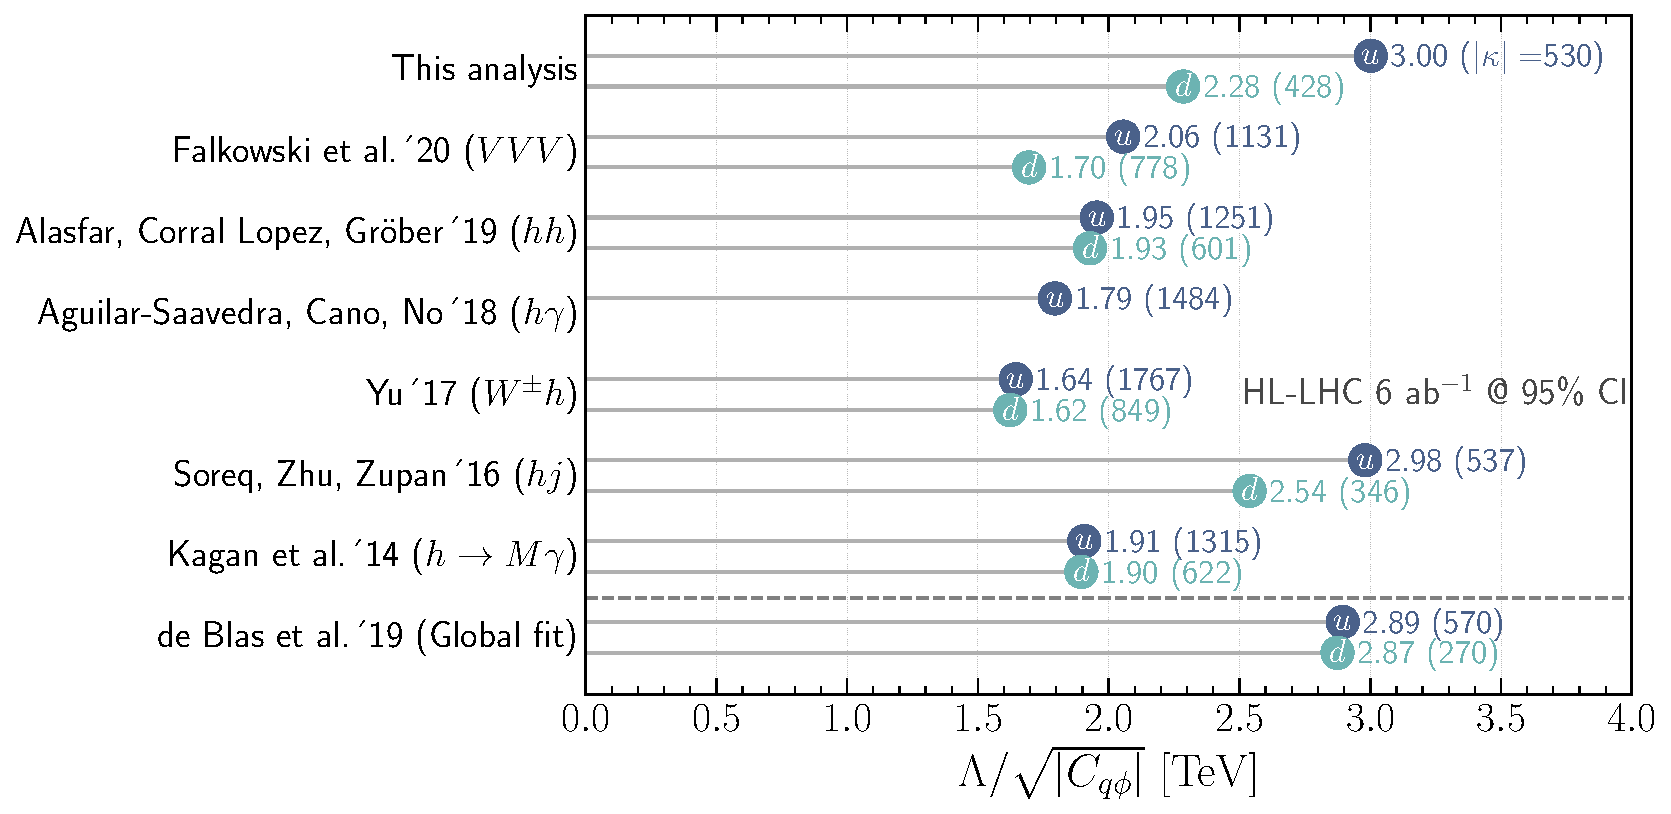
\includegraphics[width=\linewidth]{fig/ueberblick.pdf}
	\caption{Summary of the $95\%$ CI/CL sensitivity bounds on the SMEFT Wilson coefficients $C_{u\phi}$ (blue), and $C_{d\phi}$ (green). The bounds are interpreted in terms of the NP scale $\Lambda$ that can be reached through the measurements of the Wilson coefficient at the HL-LHC at $6$ \invab, the corresponding $\kappa_q$'s are shown inside the parentheses. Single parameter fit $95\%$ CI bounds are used from this analysis for comparison with previous studies.}
	\label{fig:comparison}
\end{figure}

One of the main features of the effective couplings $hh q\bar q$ and $hhh q\bar q$ emerging from SMEFT operator $\mathcal O_{q\phi}$, or the Chiral Lagrangian for that matter, is that these couplings are either free from propagator suppression for $hh q\bar q$ or scale with energy for $hhh q\bar q$ while being safe from strong unitarity constraints. This feature gives processes with multiple Higgs and/or vector bosons $V= W^\pm, Z$ an advantage in constraining $\mathcal O_{q\phi}$. The latter constrains come from the longitudinal degrees of freedom of the gauge bosons  which can be understood from the Goldstone boson equivalence theorem. The use of the final state $VV$ as a probe for $\mathcal O_{q\phi}$ is difficult due to the large SM background. However, the three-boson final state $VVV$ was shown to give strong projected bounds for light-quark Yukawa couplings for HL-LHC with 95\% CL bounds on $\kappa_u \sim 1600$, and $\kappa_d\sim 1100$. A ten fold improvement is expected at FCC-hh~\cite{Falkowski:2020znk} with bounds of order $\kappa_d\sim 30$. 
Higgs pair production has a smaller SM background compared to $VV$ production, but it has a significantly smaller cross section too, even when compared to $VVV$, as the latter process has already been observed at the LHC~\cite{Sciandra:2688061,CMS-PAS-SMP-19-014}.

On the contrary, Higgs pair production is inaccessible with the runs I-III of the LHC, but it is potentially accessible at the HL-LHC~\cite{Binoth:2006ym} having a $ \sigma \cdot BR\sim 1\mathrm{fb}^{-1}$. However, Higgs pair production, particularly the channel $h \to b \bar b \gamma \gamma $, is of significant interest as it has unique features. The first being the ability to constrain the trilinear and light-quark Yukawa couplings simultaneously, as we show in this work. Secondly, Higgs pair production could probe non-linear relations between Yukawa interaction and $hh q\bar q$ couplings~\cite{Contino:2012xk,Alasfar:2019pmn}. Lastly, Higgs pair production is expected to be significant enhanced in certain models involving modification of light-quark Yukawa couplings (cf. ~\cite{Bar-Shalom:2018rjs,Bauer:2017cov,Egana-Ugrinovic:2021uew})

For future colliders, like the FCC-hh at $100$ TeV, in addition to Higgs pair production triple Higgs production might be an interesting channel for constraining the operators with Wilson coefficient $C_{u\phi}$ and $C_{d\phi}$ due to the energy increase of a Feynman diagram coupling the quarks to three Higgs bosons.   In this case, a similar study to ours should be performed to see whether also in this case it will be important to do a combined fit on the light quark Yukawa couplings together with the trilinear and quartic Higgs self-couplings.\footnote{In~\cite{Papaefstathiou:2047255}, it was shown that $\sim \mathcal{O}(1)$ bounds on the quartic Higgs self-coupling can be reached at the FCC-hh.}

Finally, we note that there are also non collider signatures for enhanced light-quark Yukawa couplings, manifesting in frequency shifts in atomic clocks from Higgs forces at the atomic level~\cite{Delaunay:2016brc}. 